% !TEX root = ../Dokumentation.tex
\subsection{Intelligente Systeme}

\subsubsection{Software auf Mini-Computer}
Das Softwarekonzept basiert auf dem MVC\footnote{MVC = Model-View-Control}-Prinzip, wobei sich die View auf einen reinen Debug-Zweck beschränkt. Der Controller kommunziert mit allen Subprozessen und grenzt an die Schnittstelle zur Hardwaresteuerung. Um die Performance des Rasperry Pi möglichst auszunutzen wird mit Threads gearbeitet. Die parallel laufenden Subprozesse sind:

\begin{itemize}
\item Bilderzeugung,
\item Objekterkennung und
\item Fahrbahnerkennung.
\end{itemize}
Zusätzlich wurden auch die Debug-View und die UART-Kommunikation zum Teil als Threads implementiert.
\begin{figure}[H]
	\centering
	\includegraphics[width=0.8\textwidth]{03_Loesungskonzept/pictures/grobablauf.png}
	\caption{Aktivitätendiagramm Grobablauf}
\end{figure}

Der Zustand des Fahrzeuges wird im Model gespeichert und steht allen Prozessen zur Verfügung. Die Datenstruktur ist dabei so aufgebaut, dass keine Zugriffskonflikte entstehen sollten.\\
Der Controller behandelt alle Anweisungen der Prozesse. Meldet beispielsweise die Objekterkennung einen Container, hat dieser Priorität vor dem normalen Fahren und das Mikrocontroller-Board erhält die entsprechenden Anweisungen und kann jederzeit die Kontrolle übernehmen. Das folgende Diagramm zeigt eine Gesamtübersicht von den verschiedenen Komponenten.\\[0.2cm]
\begin{figure}[H]
\centering
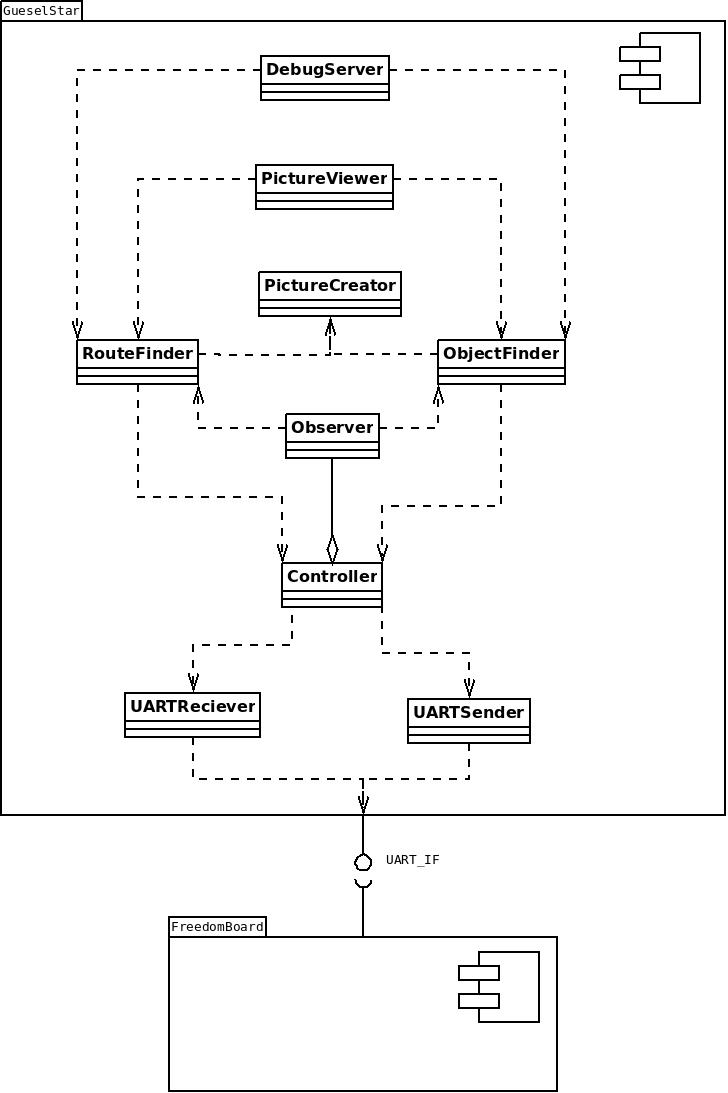
\includegraphics[width=0.8\textwidth]{03_Loesungskonzept/pictures/Komponentendiagramm_detailliert_v2.jpeg}
\caption{Komponentendiagramm}
\end{figure}
Damit keine zyklischen Abhängigkeiten enstehen, wurde entschieden, dass ein Oberserver nach dem Observer-Entwurfsmusster (GoF) implementiert wird. Normalerweise senden der RouteFinder und der ObjectFinder die Informationen an den Controller. Beim Eintreffen an der Kreuzung zum Beispiel, muss aber der Controller Informationen an den ObjectFinder senden. Diese Informationen werden über den ObjectStateObserver gesendent, wobei sich der ObjectFinder zuerst beim Controller als Observer registrieren muss.

\textbf{Debug-View}\\[0.2cm]
Um während der Implementierungs-Phase der geschriebene Code zu testen wurde eine Debug-View entwickelt. Mit dieser kann auf den Debug-Server, welcher auf dem Raspberry Pi gestartet wird, zugegriffen werden. Nach einer erfolgreichen Verbindung werden die aufgenommenen Bilder vom Server an den Client (GueselStarObserver) gesendet.

\begin{figure}[H]
\centering
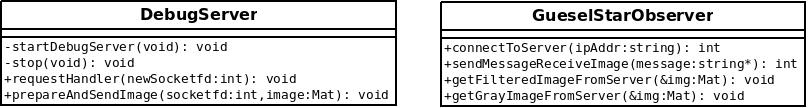
\includegraphics[width=0.8\textwidth]{03_Loesungskonzept/pictures/DebugView.jpeg}
\caption{Debug-View}
\end{figure}

Die Kommunikation zwischen Server und Client läuft über TCP/IP. Auf dem Server wird ein Server-Socket geöffnet, auf welches sich der Client verbinden kann.

Zusätzlich werden über die Konsole der SSH-Verbindung Werte ausgegeben. Dazu wurde die Bibliothek ncurses verwendet, welche es ermöglicht Daten schön übersichtlich und gruppiert darzustellen.

\textbf{Konfiguration}\\[0.2cm]
Neu geschriebener Code benötigt einen erneuten Build. Um einen neuen Build, welcher Zeit benötigt, zu unterbinden wurde eine Konfigurations-Datei erstellt, in welcher alle benötigten Parameter angepasst werden können. Das Einlesen der Konfiguration erfolgt über einen selbstentwickelten Parser und wird anschliessend in einem Objekt der Klasse "{}PRENConfiguration"{} abgespeichert.

\begin{figure}[H]
\centering
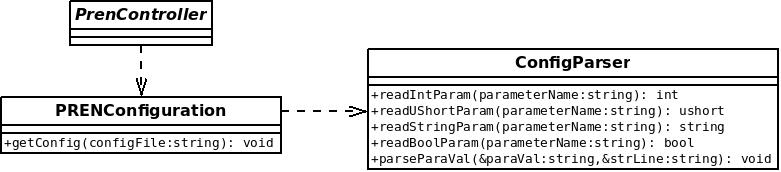
\includegraphics[width=0.8\textwidth]{03_Loesungskonzept/pictures/Configuration.jpeg}
\caption{Konfiguration}
\end{figure}

\textbf{Vergleich Konzept und Umsetzung}\\[0.2cm]
Die Planung der Softwarearchitektur war nach Pren1 noch nicht weit fortgeschritten, daher wurden die meisten Entscheidungen erst in Pren2 getroffen. Die parallelisierte Ausführung der Threads "{}Fahrbahnerkennung"{}, "{}Objekterkennung"{} und "{}Bilderzeugung"{} wurde beibehalten, jedoch kamen noch einige Threads, wie die Klassen für die UART-Kommunikation dazu.
 
%***************************
\subsubsection{Software auf Mikrocontrollerboard}

\textbf{SW Architektur}\\[0.2cm]
Auf dem Mikrocontroller (Freedomboard KL25Z) wurde mit dem Betriebssystem FreeRTOS gearbeitet. Dies ermöglicht die Erstellung von verschiedenen Tasks. Dies erlaubt eine bessere Trennung der einzelnen Softwarekomponenten und erleichtert das Programmieren. Die verschiedenen Tasks wurden bereits im PREN1 geplant und nun im PREN2 umgesetzt. 
Hier eine Übersicht der Tasks und Events:

\begin{figure}[H]
	\centering
	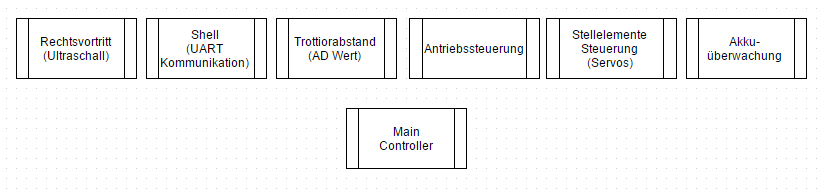
\includegraphics[width=0.9\textwidth]{03_Loesungskonzept/pictures/MC_Tasks.png}
	\caption{Übersicht MC Tasks}
\end{figure}
In den folgenden Abschnitten werden kurz auf die einzelnen Tasks und Events eingegangen. Dies dient jedoch nur der Übersicht.\\
\textbf{Controller}\\[0.2cm]
Dieser Task steuert das Freedomboard. Das heisst konkret, dass dieser Task das initialisieren, fahren, aufladen, entladen  und beenden des Programmes zuständg ist. Dies ist über eine FineState Maschiene realisiert, welche bei besonderen Events den State wechselt. Ein besonderer Event ist zum Beispiel das Startkommando über die Kommunikation oder eine Unterspannung am Akku.\\[0.2cm]
\textbf{Kommunikation}\\[0.2cm]
Dieser Task übernimmt die Auswertung der erhaltenen Kommandos über die UART Schnittstelle. Dies geschieht über eine sogenannte Parsertabelle. In dieser Parsertabelle können beliebig weitere Kommandos (Funktionen) hinzugefügt werden. Dieser Task wird alle 10ms aufgerufen, da die Kommunikation mit dem Raspberry Pi möglichst schnell funktionieren soll.\\[0.2cm]
\textbf{Analog-Digitalwandlung}\\[0.2cm]
Dieser Task holt und verarbeitet die Daten aus dem Analog Digitalwandler des KL25Z. Das heisst konkret, es werden beide Akku Spannungen ausgelesen und überwacht. Zudem wird der Widerstandswert des Flexsensensors eingelesen und damit der Abstand zum Gehsteig berechnet. Zur Akkuüberwachung folgen weiter im Text weitere Informationen.\\[0.2cm]
\textbf{Geschwindigkeitsregelung}\\[0.2cm]
Der Geschwindigkeitsregelungstask regelt die Geschwindigkeit des DC-Antriebmotors. Dies geschieht über einen PID Regler. Dieser wurde vom Modul Mikrocontrollertechnik an der Hochschule Luzern übernommen und nach den eigenen Bedürfnissen angepasst.\\[0.2cm]
\textbf{Ultraschall}\\[0.2cm]
Dieser Task steuert den Ultraschallsensor an. Dies wurde nach einem Tutorial von mcuoneclipse.com realisiert und auf die Softwareumgebung noch weiter angepasst.\\[0.2cm]
\textbf{Master check}\\[0.2cm]
Dieser Task ist die Lebensversicherung des Fahrzeugs. Hier wird überprüft ob der Master (Raspberry Pi) noch angeschlossen und Funktionstüchtig ist. Wenn das Mikrocontrollerborad nicht innerhalb von wenigen Sekunden eine Bestätigungsmeldung des Masters bekommt, wird das Freedomboard in den Beendet Modus wechseln und fährt somit nicht unkontrolliert herum. \\[0.2cm]
\textbf{Analog Digitalwandlung}\\[0.2cm]
Hier wird die Akkuspannung und der Flexsensorwert eingelesen und verarbeitet. Wenn nun die Akkuspannung zu niedrig ist, wird dies in diesem Task detektiert. Zudem wird hier der Spannungwert über dem Flexsensor in mm Abstand zum Trottoir umgerechnet.\\[0.2cm]
\textbf{Event}\\[0.2cm]
Die Events treten unregelmäßig und ungeplant auf. Diese unterbrechen das normale Programm (Interrupt) und führen einen eigenen kurzen Programmcode aus. Dies ist bei den im Bild aufgeführten Funktionen der Fall.\\[0.2cm]
\textbf{Die Konfigurationsdatei}\\[0.2cm]
Damit einzelne Komponenten des Fahrzeuges getestet werden konnten, mussten teilweise andere Fahrzeugkomponenten ausgeschaltet werden. Zum Beispiel als das Aufladen des Containers getestet werden sollte, wollte man nicht noch das Anfahren testen. Aus diesem Grund ist das File config.h entstanden. Darin lassen sich einzelne Baugruppen und Funktionen des Programmes effizient ein oder ausschalten. Dieses System hat sich als sehr nützlich erwiesen und ist sehr wichtig für die Funktion des Fahrzeuges.\\[0.2cm]
\textbf{Das Debuggen und Fehlersuchen}\\[0.2cm]
Ein grosser Vorteil am Freedomboard ist die Möglichkeit zum Debuggen. Dies war einerseits über die normale Entwicklungsumgebung Kinetis möglich. Andererseits war dies auch durch den SystemViewer möglich. Damit man dieses Tool nutzen kann, ist es nötig den Debugger von der Firma Segger zu brauchen. Mit diesem Tool kann analysiert werden, wie viel und wie lange ein Task aktiv ist. Diese Tool half dabei, schwierige Fehler im Taskhandling zu finden. Eine Anleitung dazu findet sich auch auf mcuoneclipse.com.\\[0.2cm]
\textbf{Vergleich Konzept und Umsetzung}\\[0.2cm]
Die Software wurde grösstenteils so implementiert, wie dies im Pren1 geplant war. Die einzigen Unterschiede zwischen dem Konzept und der Umsetzung liegen in der Zusammenführung verschiedener Tasks. So wurde die Tasks Akkuüberwachung und Trottoirabstand zu dem Task Analogdigitalwandlung zusammengeführt. Dies weil so das Programm effizienter gemacht werden konnte. Zudem wurde der Task Stellelementesteuerung nicht als Task, sondern als Event realisiert. Dies weil zum Beispiel das neue Stellen eines Servos immer eine eingabe erfordert und somit ein Event viel sinnvoller ist als polling. 
%***************************
\subsubsection{Schnittstellen}
\textbf{UART Schnittstelle}\\[0.2cm]
Aufgabe der UART Schnittstelle ist es, die Kommunikation zwischen Minicomputer und Mikrocontroller sicherzustellen. Dazu gehören folgende Aufgaben
\begin{itemize}
\item Austausch der Sensorwerte für die Regelkreise.
\item Definierte Kommandos um die Aktoren anzusteuern.
\end{itemize}
\textbf{Architektur und Designentscheide}\\[0.2cm]
Um den Datenfluss einfach zu halten, werden Sensorwerte periodisch vom Freedom Board an das Raspberry Pi übertragen. Die Klasse \code{UARTReciever} ist entsprechend als Thread realisiert entschlüsselt den empfangenen String und schreibt den Wert auf entsprechende Member-Variabeln. Diese können über Funktionsgerechte Get-Methoden abgefragt werden.\\
Das Senden von Daten wird ebenfalls über Funktionsgerechte Send-Methoden von der Klasse \code{UARTSender} zur Verfügung gestellt. Entsprechend setzen diese Methoden die Ausgabestrings zusammen.\\[0.2cm]
\textbf{UART-Methodenstrings}
\begin{figure}[H]
	\centering
	\begin{tabular}{|l|l|l|l|l|} \hline
	Aktion/Aktor         & Richtung     & String,[params]    & Übergabewert              & Bemerkungen \\\hline\hline
	Ultraschall          & Frd$\to$Rasp & Ul,uint16          & distance cm               & periodisch all 0.3s \\\hline
	Flexsensor1 und ev 2 & Frd$\to$Rasp & Fld1,uint8         & distance mm               & periodisch all 0.2s \\\hline
	StatusAuf            & Rasp$\to$Frd & StA d,uint16       & distance mm               & \\
	                     & Frd$\to$Rasp & StAf               &                           & Wenn  abgeschlossen \\\hline
	StatusAb	             & Rasp$\to$Frd & StE d,uint16       & distance mm               & \\
	                     & Frd$\to$Rasp & StEf               &                           & Wenn abgeschlossen\\\hline
	DC Motor             & Rasp$\to$Frd & DCDr d,uint8,uint8 & mm pro sek.,modus         & Modi: hard/soft \\
	                     & Frd$\to$Rasp & DCDr,uint8         & mm pro sek.               & wenn encoder say o \\\hline
	Lenkungsservo        & Rasp$\to$Frd & LeS p,uint8        & abs Winkel (0=127)        & \\\hline
	Kameraservo          & Rasp$\to$Frd & CamP p,uint8       & Kamera pos                & \\\hline
	Debug Messages       & Frd$\to$Rasp & DBG,char[]         & Meldung                   & \\\hline
	NochDa               & Frd$\to$Rasp & There              & Flag                      & periodisch all 0.5s \\
	                     & Rasp$\to$Frd & Ja a               & Erhalten?                 & Wenn nein $\to$ DC stop \\\hline
	Start                & Rasp$\to$Frd & StartFrd a         &                           & Hochfahren und init \\
	                     & Frd$\to$Rasp & Ready              &                           & \\\hline
	Stop	                 & Rasp$\to$Frd & Stop a             &                           & Programm beenden \\
		                 & Frd$\to$Rasp & Stop               &                           & Programm beendet \\ \hline
	\end{tabular}
	\caption{Definition der Übertragungsstrings}
\end{figure}
\textbf{Methodenübersicht \code{UARTReciever}}
\begin{itemize}
\item \code{int getFlexDistance(void)} Methode, die den Abstand des Flexsensors zurückgibt.
\item \code{int getEngineSpeed(void)} Methode, die des Antriebsmotors aktuelle Geschwindigkeit zurückgibt.
\item \code{int getUltraDist(void)} Methode liefert die kürzeste Distanz des Ultraschallsensors zurück.
\end{itemize}
\textbf{Methodenübersicht \code{UARTSender}}
\begin{itemize}
\item \code{bool sendStartCmd(void)} Methode, die das Freedom Board aktiviert und alle Aktoren in Ausgangsposition bringt. Rückgabe: \code{false}, wenn ein Übertragungsfehler aufgetreten ist, \code{true} sonst.
%
\item \code{bool sendStopCmd(void)} Methode, welche dem Freedom Board das Ende des Programms signalisiert.  Rückgabe: \code{false}, wenn ein Übertragungsfehler aufgetreten ist, \code{true} sonst.
%
\item \code{bool setCameraPos(ushort pos)} Methode dreht die Kamera auf die gewünschte Position. Übergabewerte aus \code{PrenController} um ungültige Werte zu vermeiden:\\
\code{CAM\_STRAIGHT} = gerade, \code{CAM\_CHECK\_STREET} für Rechtsvortritt, \code{CAM\_TURN\_RIGHT} = Rechtskurve und \code{CAM\_TURN\_LEFT} = Linkskurve. Rückgabe: \code{false}, wenn ein Übertragungsfehler aufgetreten ist, \code{true} sonst.
%
\item \code{bool setEngineSpeed(uint8\_t speed, EngineModesE mode = SOFT)} Methode setzt den Motor auf die gewünschte Geschwindigkeit, der Modus kann zwischen \code{SOFT} (default) und \code{HARD} gewählt werden. \code{HARD} = Notfall. Rückgabe: \code{false}, wenn ein Übertragungsfehler aufgetreten ist, \code{true} sonst.
%
\item \code{bool setContainerFound(uint16\_t distance)} Methode teilt dem Mikrocontroller mit, einen Container gefunden zu haben. Übergabeparameter: Abstand zum Container. Rückgabe: \code{false}, wenn ein Übertragungsfehler aufgetreten ist, \code{true} sonst.
%
\item \code{bool setTargetFieldFound(uint16\_t distance)}  Methode teilt dem Mikrocontroller mit, das Ziel gefunden zu haben. Übergabeparameter: Abstand zum Zielfeld. Rückgabe: \code{false}, wenn ein Übertragungsfehler aufgetreten ist, \code{true} sonst.
%
\item \code{bool setSteering(uint8\_t steeringAng)}  Methode teilt dem Mikrocontroller mit, das auf einen bestimmten Winkel gelenkt werden soll. 0 Grad = 127 aufgrund des unsigned Typen. Übergabeparameter: Winkel, auf den die Lenkung gestellt werden soll. Rückgabe: \code{false}, wenn ein Übertragungsfehler aufgetreten ist, \code{true} sonst.
%
\item \code{bool stillThereResponse(void)} Methode sendet ein Ja auf die Frage, ob die Verbindung noch steht.  Rückgabe: \code{false}, wenn ein Übertragungsfehler aufgetreten ist, \code{true} sonst.
\end{itemize}